% !TeX root = ../main.tex

    \begin{frame}{Performances of Different Policies}
        \scriptsize
        $M =4$, $\delta =1$, $N =10$, $L_j =21, j \in \mathcal{N}$, $p_0 = 0$, $|\Omega| = 1000$.
        \begin{table}[ht]
          \centering
          \begin{tabular}{|l|l|l|l|l|l|l|}
          \hline
           T & Probabilities & DSA (\%) & DP1 (\%) & Bid (\%) & Booking (\%) & FCFS (\%) \\
          \hline
          60  & [0.25, 0.25, 0.25, 0.25]  & 99.12 & 98.42 & 98.38 & 96.74 & 98.17 \\
          70  &   & 98.34 & 96.87 & 96.24 & 97.18 & 94.75 \\
          80  &   & 98.61 & 95.69 & 96.02 & 98.00 & 93.18 \\
          90  &   & 99.10 & 96.05 & 96.41 & 98.31 & 92.48 \\
          100 &   & 99.58 & 95.09 & 96.88 & 98.70 & 92.54 \\
          \hline
          60  & [0.25, 0.35, 0.05, 0.35]  & 98.94 & 98.26 & 98.25 & 96.74 & 98.62 \\
          70  &   & 98.05 & 96.62 & 96.06 & 96.90 & 93.96 \\
          80  &   & 98.37 & 96.01 & 95.89 & 97.75 & 92.88 \\
          90  &   & 99.01 & 96.77 & 96.62 & 98.42 & 92.46 \\
          100 &   & 99.23 & 97.04 & 97.14 & 98.67 & 92.00 \\
          \hline
          60  & [0.15, 0.25, 0.55, 0.05]  & 99.14 & 98.72 & 98.74 & 96.61 & 98.07 \\
          70  &   & 99.30 & 96.38 & 96.90 & 97.88 & 96.25 \\
          80  &   & 99.59 & 97.75 & 97.87 & 98.55 & 95.81 \\
          90  &   & 99.53 & 98.45 & 98.69 & 98.81 & 95.50 \\
          100 &   & 99.47 & 98.62 & 98.94 & 98.90 & 95.25 \\
          \hline
          \end{tabular}
        \end{table}
        DSA has better performance than other policies under different demands.

    \end{frame}
      
    \begin{frame}{Impact of Social Distancing as Demand Increases}
      \vspace{-0.4cm}
      % \begin{figure}[h]
      %   \centering
      %   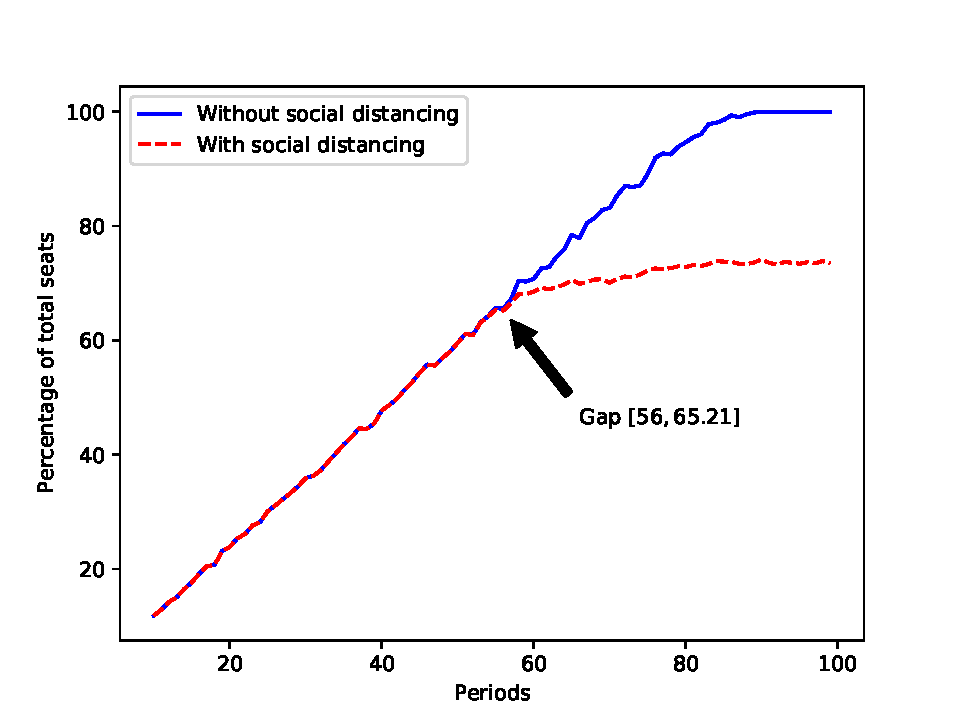
\includegraphics[width=0.5\textwidth]{./images/p1.pdf}          
      %   \caption{When probability is [0.25, 0.25, 0.25, 0.25]}
      %   \end{figure}
        

      \begin{columns}
        \column{6cm}  %第一栏(左栏)宽度为5cm
          \begin{figure}[ht]
            \centering
            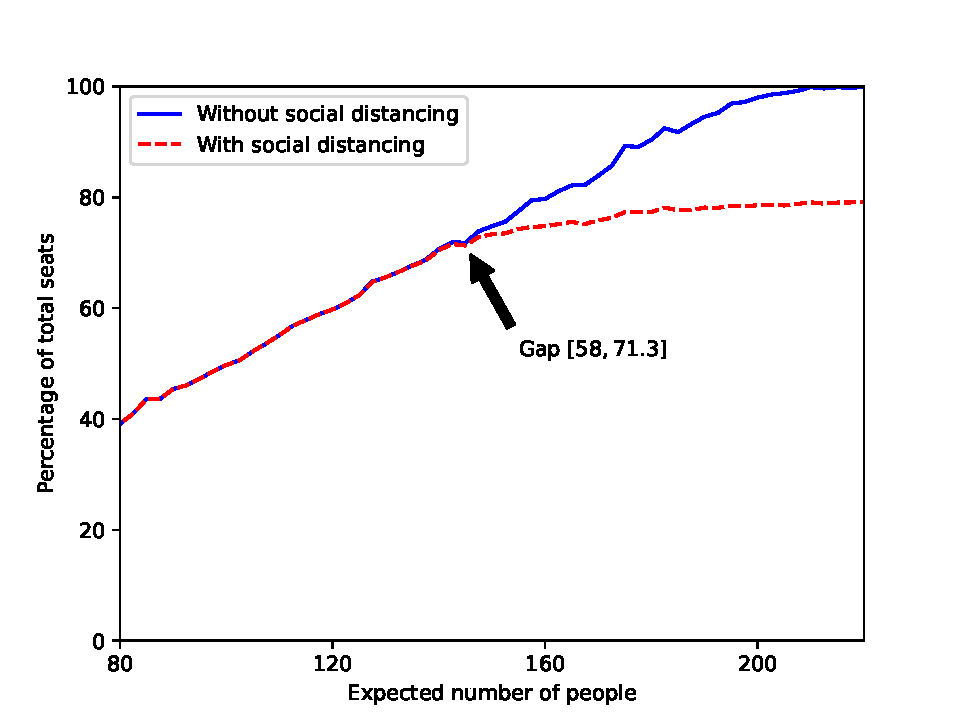
\includegraphics[width = 1\textwidth]{./images/without2.pdf}
          \end{figure}
          \column{6cm}
          \scriptsize
          \begin{figure}[ht]
            \centering
            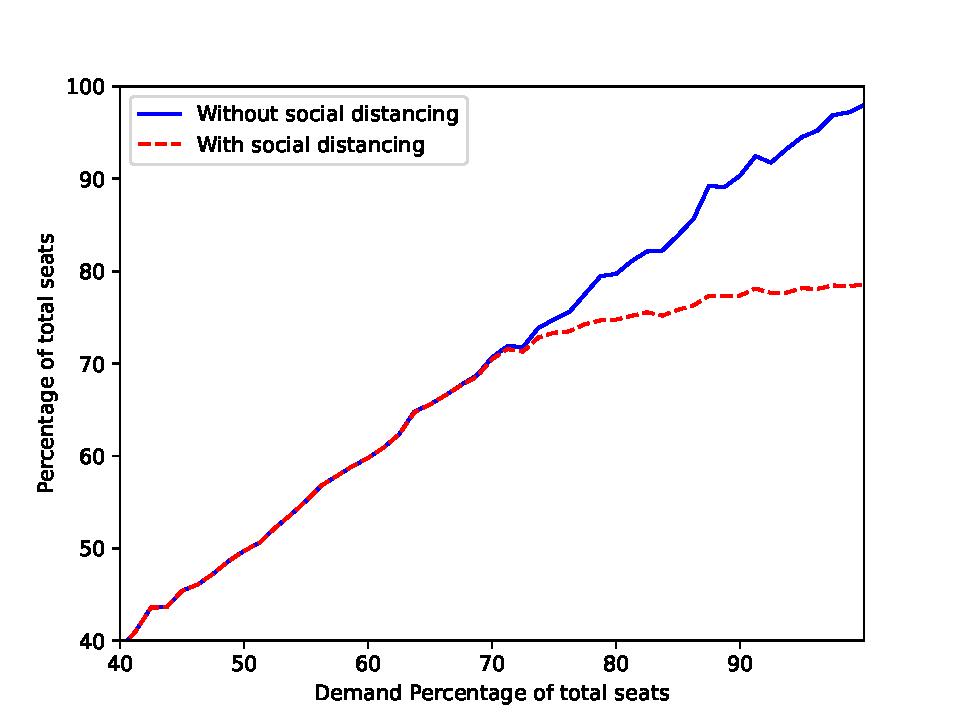
\includegraphics[width = 1\textwidth]{./images/without1.pdf}
          \end{figure}
      \end{columns}
      % The gap point represents the first period where the number of people without social distancing is larger than that with social distancing and the gap percentage is the corresponding percentage of total seats.
      \begin{itemize}
        \item Gap point: the first period when there is difference 
        \item Demand less than 71.3\% total seats: no difference
        \item Demand larger than 71.3\% total seats: the difference becomes larger
      \end{itemize}
  \end{frame}

    \begin{frame}{Estimation of Gap Point}
      \scriptsize
      $\gamma = p_1 * 1 + p_2 * 2 + p_3 * 3 + p_4 * 4$: the expected number of people at each period.
      \begin{columns}
        \begin{column}{0.8\textwidth}
      \begin{figure}[ht]
        \centering
        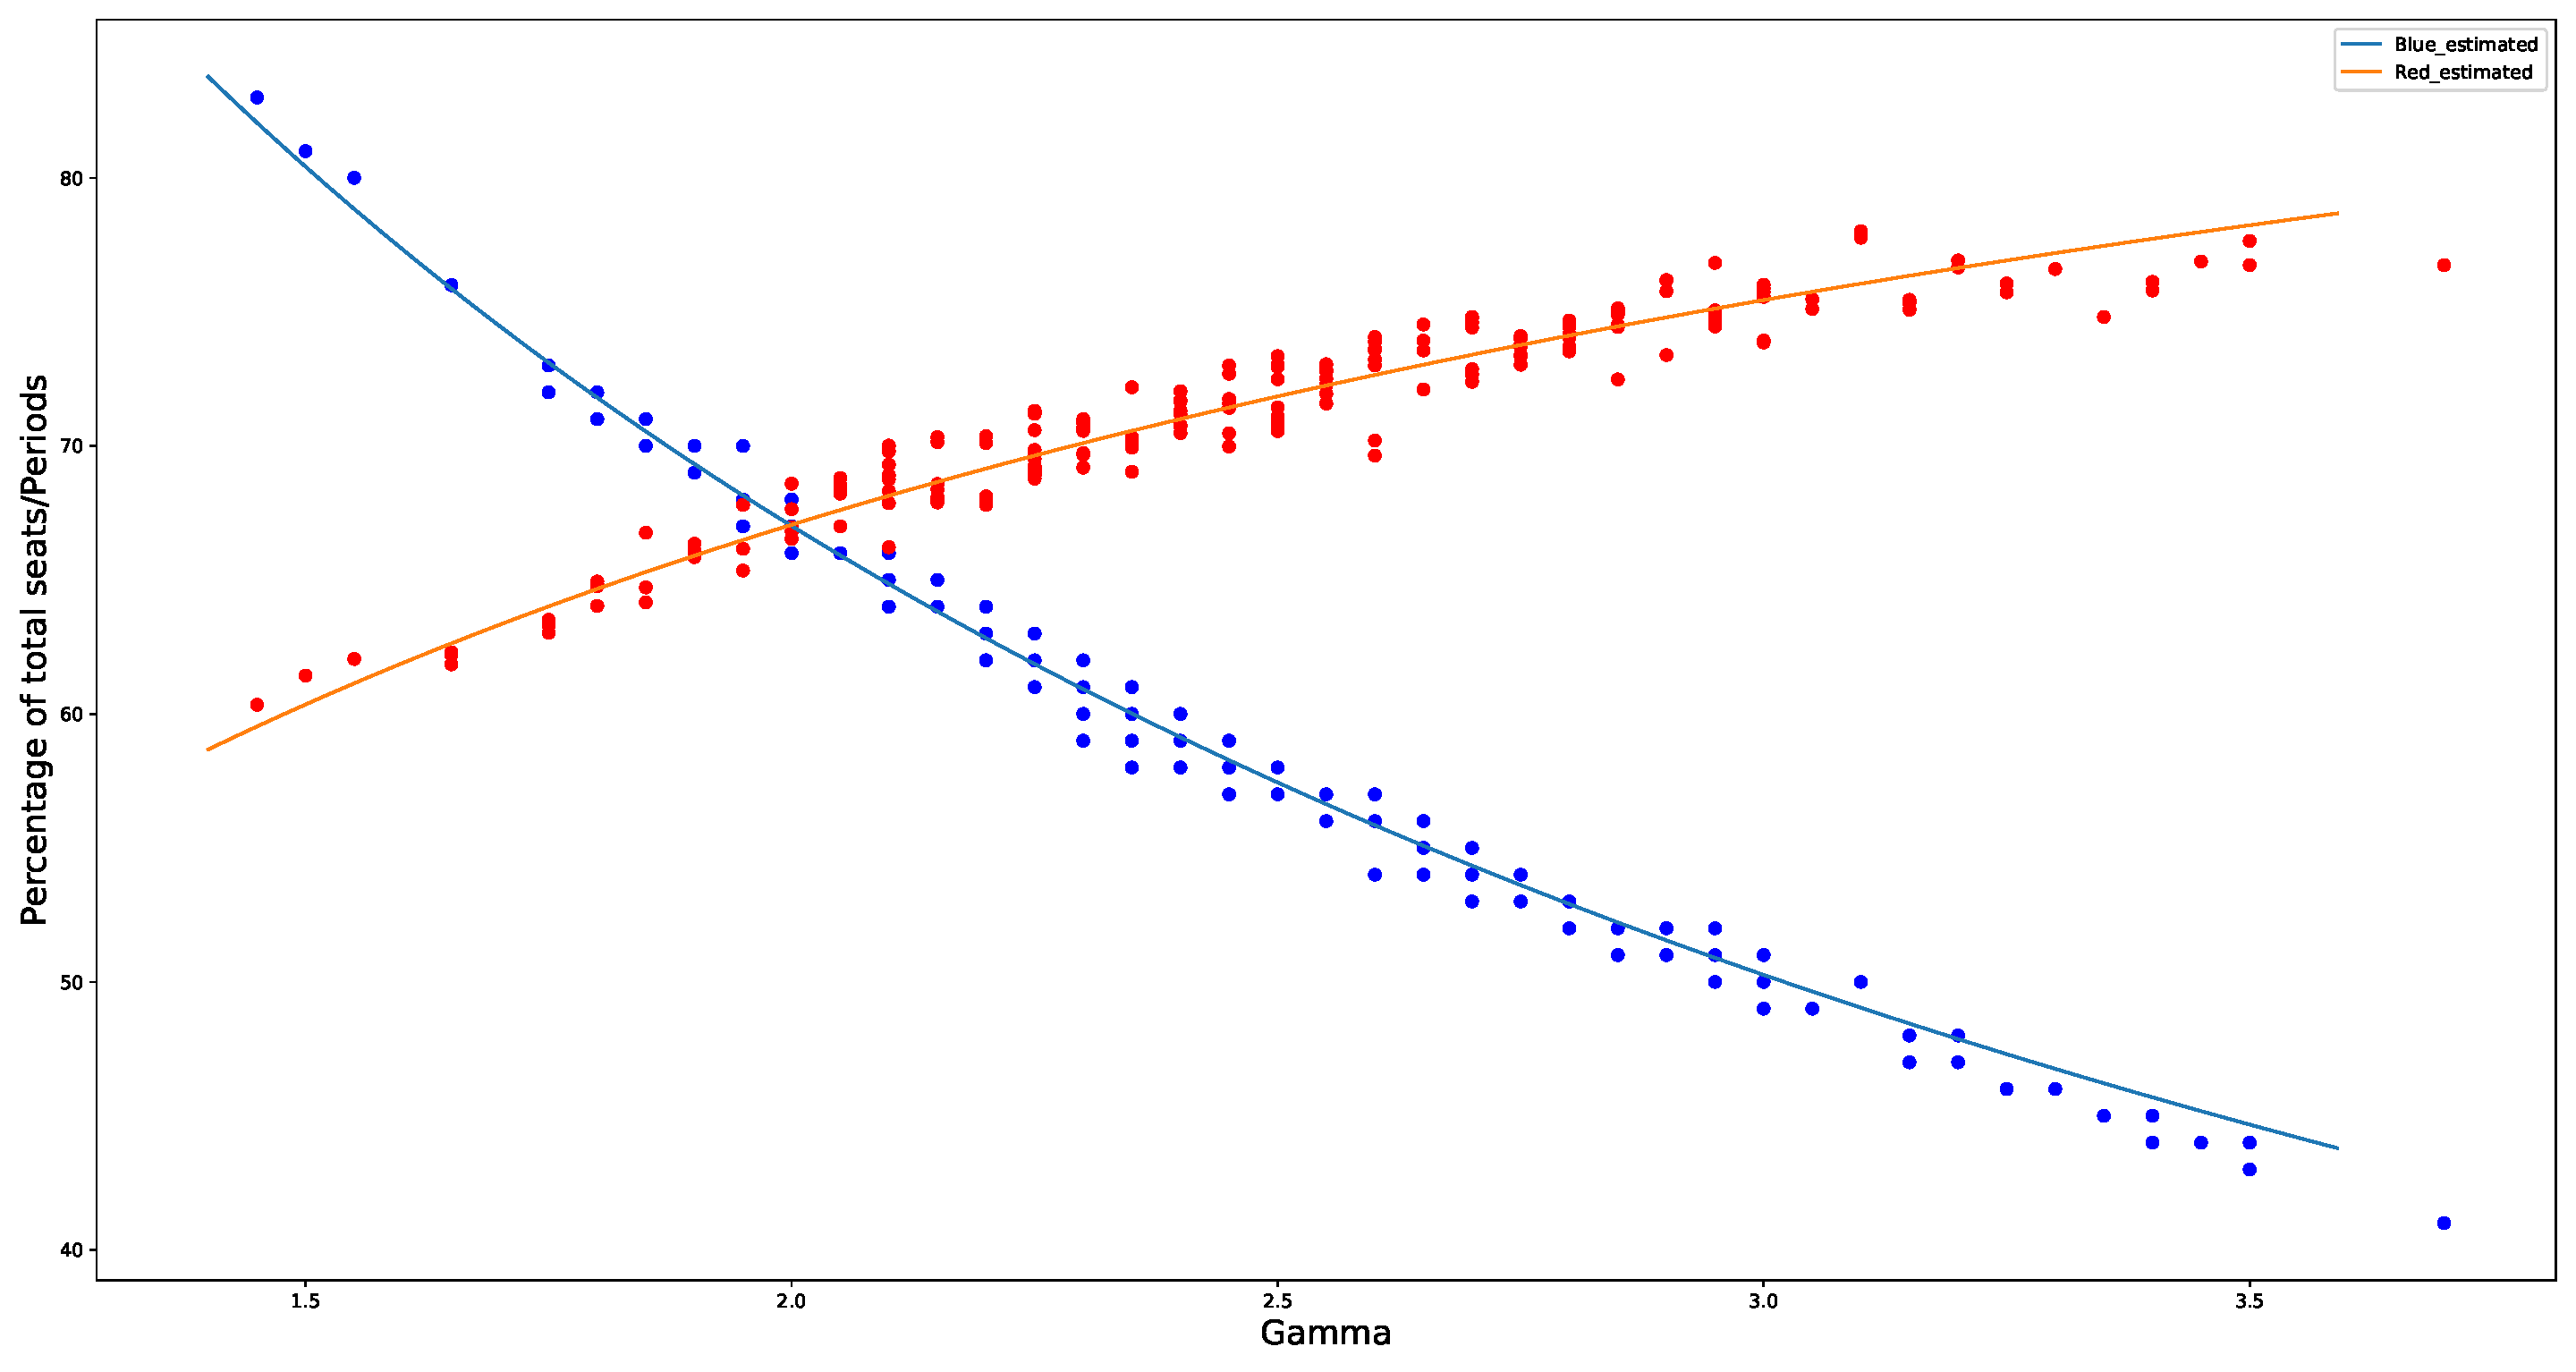
\includegraphics[width = 1\textwidth]{./images/gamma.pdf}
        \captionsetup{font={scriptsize}}
        \caption{Gap points with 200 probabilities}
    \end{figure}
  \end{column}

  \begin{column}{0.2\textwidth}
    Assumption: the groups before gap point will occupy all seats.
    $c_1, c_2$ can be seen as the discount factor compared to the ideal assumption.

    {\color{blue} $y_1 = \frac{c_1 \tilde{L}}{\gamma + \delta}$}
    {\color{red}  $y_2 = c_2 \frac{\gamma}{\gamma + \delta} \frac{\tilde{L}}{\tilde{L}-N \delta}$}
  \end{column}
  \end{columns}

    \scriptsize
    {\color{blue} Blue points}: period of the gap point.
    {\color{red} Red points}: occupancy rate of the gap point. 
    Gap points can be estimated with $\gamma$. Different seat layout affects $c_1, c_2$. The larger $c_1, c_2$, the closer to the ideal assumption.
    \end{frame}

  %   \begin{frame}{Impact of Social Distancing as Demand Increases}


  % \end{frame}

    % We simulate 200 probabilities. For each probability, we run 100 instances to calculate the gap point and the corresponding occupancy rate on average. 
    
    % The point in the figure is the average of 100 instances.
    % x-axis is gamma, y-axis is periods/ and occupancy rate.

    % \begin{frame}{Seat Assignment under Fixed Seat Planning}
    %   % To evaluate the effectiveness of the initial seat planning, we employ a dynamic situation where decisions are made based on real-time feedback. In this context, we utilize a fixed seat planning as the foundation, and then make informed decisions accordingly.
    %   \small
    %   \begin{itemize}
    %     \item Group-type Control
    %     \item[-] Suppose the corresponding supply is $[X_1, \ldots, X_M]$. ($X_{i} = \sum_{j} x_{ij}, \forall i$)
        
    %     For the arrival of group type $i$,
  
    %     \item[-] if $X_i > 0$, accept it directly, assign it the seats planned for group type $i$;
    %     \item[-] if $X_i = 0$, determine which group type to accept it.
    %   \end{itemize}
  
    %   \vspace{-0.5cm}
  
    %   \begin{figure}[h]
    %     \centering
    %     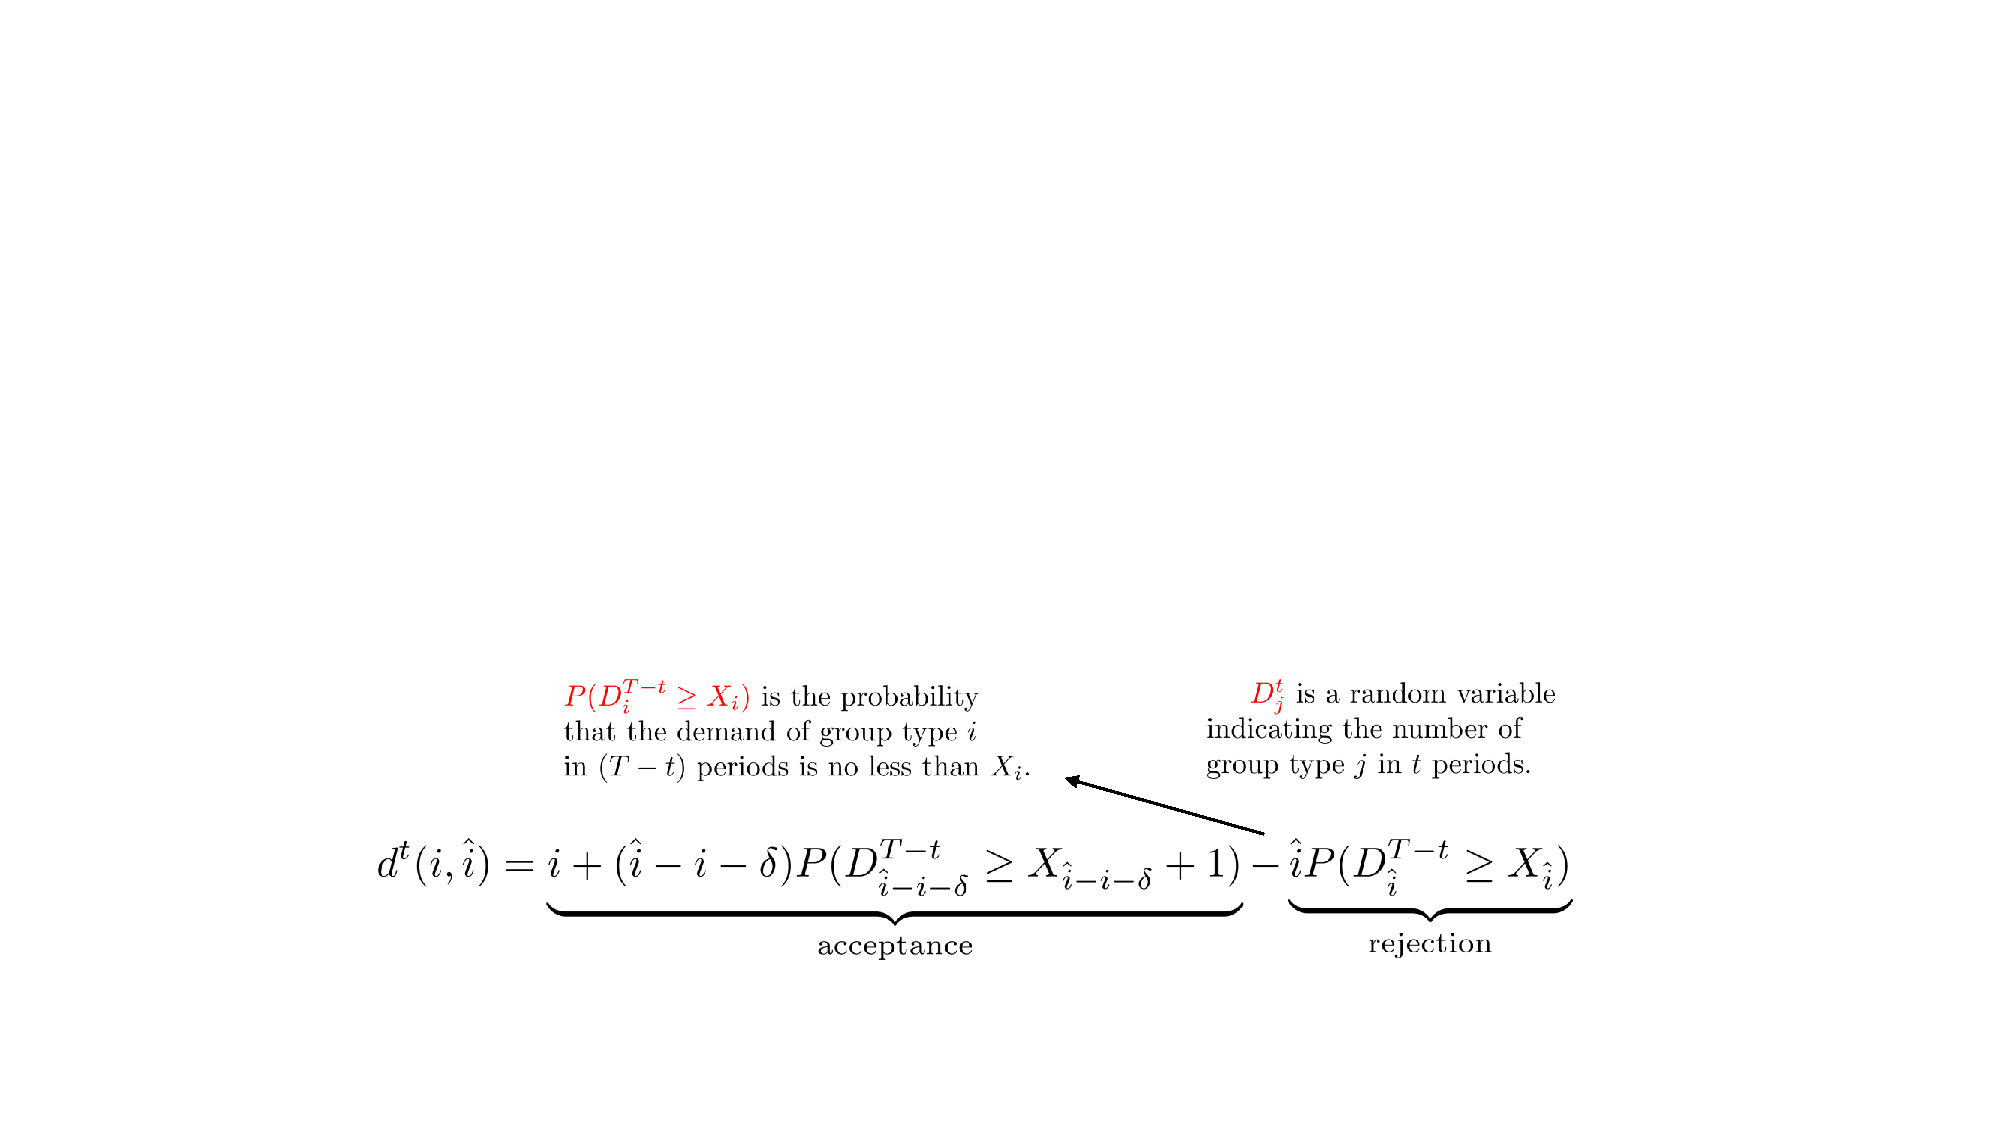
\includegraphics[width = 0.8\textwidth]{./images/group_type.pdf}
    %   \end{figure}
  
    %   \vspace{-0.1cm}
  
    %   For all $\hat{i} > i$, find the maximum value denoted as $d^{t}(i, \hat{i}^{*})$.
      
    %   If $d^{t}(i, \hat{i}^{*}) \geq 0$, we place the group of $i$ in $(\hat{i}^{*} + \delta)$-size seats. Otherwise, reject the group.
  
    %   % After acceptance, customers have more freedom to choose their seats with the seat planning.
    % \end{frame}
    
    \begin{frame}{Seat Assignment under Fixed Seat Planning}
      \scriptsize
      The assignment is based on the fixed seat planning and we use the group-type control to make the decision. 
      $M =4$, $\delta =1$, $L_j =21, j \in \mathcal{N}$, $p_0 = 0$, $|\Omega| = 1000$.
      \begin{table}[ht]
        \centering
        \begin{tabular}{|l|l|l|l|}
        \hline
         T & Probabilities & \# of rows & Compared to the optimal (\%)  \\
        \hline
        70  & [0.25, 0.25, 0.25, 0.25]  & 10 & 94.97  \\
        80  &   &  & 96.48   \\
        90  &   &  & 97.94   \\
        100  &   &  & 98.91   \\
        \hline
        70  & [0.25, 0.35, 0.05, 0.35]  & 10 & 95.90 \\
        80  &   &  & 97.06  \\
        90  &   &  & 98.58  \\
        100  &   &  & 99.47 \\
        \hline
        70  & [0.15, 0.25, 0.55, 0.05]  & 10 & 97.41  \\
        80  &   &  & 98.85  \\
        90  &   &  & 98.73  \\
        100  &   &  & 98.46  \\
        \hline
        140  & [0.25, 0.25, 0.25, 0.25]  & 20 & 95.83  \\
        160  &   &  & 97.46  \\
        180  &   &  & 99.05  \\
        200  &   &  & 99.74  \\
        \hline
        \end{tabular}
      \end{table}
  
    % Each entry is the average of 50 instances.
    % IP will spend more than 2 hours in some instances, as `NA' showed in the table.
    \end{frame}



    \begin{frame}{Make A Later Allocation}
      This setting is particularly applicable to larger venues, such as stadiums, where an immediate decision is made when a group arrives, but the actual allocation of seats for that group is deferred to a later time.

      \vspace{0.5cm}

      The critical part is to make the decision, thus, we choose the following policies associated with relaxation forms.

      \vspace{0.5cm}

      Policies: 

      \begin{itemize}
        \item Dynamic programming based heuristic
        \item Bid-price control
      \end{itemize}
    \end{frame}

      \begin{frame}{Performances of Different Policies}
        \scriptsize
        \begin{table}[ht]
          \centering
          \begin{tabular}{|l|l|l|l|l|l|}
          \hline
           T & Probabilities &  DP1-L (\%) & Bid-L (\%) & DP1 (\%) & Bid (\%) \\
          \hline
          60  & [0.25, 0.25, 0.25, 0.25]  & 99.52 & 99.44 & 98.42 & 98.38 \\
          70  &   & 99.32 & 98.97 & 96.87 & 96.24 \\
          80  &   & 99.34 & 99.30 & 95.69 & 96.02 \\
          90  &   & 99.55 & 99.49 & 96.05 & 96.41  \\
          100 &   & 99.78 & 99.66 & 95.09 & 96.88 \\
          \hline
          60  & [0.25, 0.35, 0.05, 0.35]  & 99.50 & 99.37 & 98.26 & 98.25  \\
          70  &   & 99.40 & 98.97 & 96.62 & 96.06 \\
          80  &   & 99.46 & 99.24 & 96.01 & 95.89 \\
          90  &   & 99.59 & 99.35 & 96.77 & 96.62 \\
          100 &   & 99.77 & 99.61 & 97.04 & 97.14  \\
          \hline
          60  & [0.15, 0.25, 0.55, 0.05]  & 99.57 & 99.54 & 98.72 & 98.74 \\
          70  &   & 99.46 & 99.39  & 96.38 & 96.90 \\
          80  &   & 99.50 & 99.30  & 97.75 & 97.87 \\
          90  &   & 99.34 & 99.44  & 98.45 & 98.69 \\
          100 &   & 99.34 & 99.55  & 98.62 & 98.94 \\
          \hline
          \end{tabular}
        \end{table}

    \end{frame}